%Author name: Aveek Podder
%Roll Number: 153070032

\documentclass[a4paper]{article}

\usepackage{amsmath}
\usepackage{graphicx}
\usepackage{float}
\usepackage{url}
\usepackage{hyperref}
\usepackage{bookmark}

\begin{document}
\title{A pendulum with friction}
\author{Aveek Podder\\
Roll number-153070032}
\date{\today}
\maketitle
\clearpage
\tableofcontents
\clearpage

\section*{Abstract}
\addcontentsline{toc}{section}{Abstract}
    In this paper we discuss the basics of oscillation of a pendulum with friction. The differential equation that represents the motion of the pendulum is solved using Scipy package of Python. This differential equation depends on different parameters like mass of the pendulum, coefficient of friction, gravity and length of the string.

\section{Introduction}
A pendulum is a weight suspended from a pivot so that it can swing freely.\cite{Miri} When a pendulum is displaced sideways from its resting, equilibrium position, it is subject to a restoring force due to gravity that will accelerate it back toward the equilibrium position. When released, the restoring force combined with the pendulum's mass causes it to oscillate about the equilibrium position, swinging back and forth. The time for one complete cycle, a left swing and a right swing, is called the period. The period depends on the length of the pendulum and also to a slight degree on the amplitude, the width of the pendulum's swing.

From the first scientific investigations of the pendulum around 1602 by Galileo Galilei, the regular motion of pendulums was used for timekeeping, and was the world's most accurate timekeeping technology until the 1930s.\cite{Marr} The pendulum clock invented by Christian Huygens in 1658 became the world's standard timekeeper, used in homes and offices for 270 years, and achieved accuracy of about one second per year before it was superseded as a time standard by quartz clocks in the 1930s. Pendulums are also used in scientific instruments such as accelerometers and seismometers. Historically they were used as gravimeters to measure the acceleration of gravity in geophysical surveys, and even as a standard of length. The word "pendulum" is new Latin, from the Latin pendulus, meaning 'hanging'.\cite{Morr}\\
The governing differential equation of pendulum motion is as follows :-
\begin{equation}\label{eq1}
    \frac{d^2\Theta}{dt^2} + \frac{b}{m}\frac{d\Theta}{dt} + \frac{g}{L}sin(\Theta) = 0
\end{equation}
In Eq.\ref{eq1} \textit{$\Theta$} represents the  angular position of the pendulum, b is the coefficient of friction, m is the mass of the pendulum, g is the acceleration due to gravity and L is the length of the string.
\section{Solving the differential equation}
The governing equation of the pendulum that is given by Eq.\ref{eq1} is solved in Python.The source code for solving the governing equation of oscillation of a pendulum with friction is available in \url{https://github.com/HisokaMorow/SDES_Project1.git}.

For this the following packages are required 
apart from \textbf{Python 2.7.12}.
\begin{itemize}
    \item{numpy 1.11.1} - all the solutions of the equation are to be stored in array format which becomes available via this package
    \item{scipy 0.18.1} - the Ordinary Differential Equation solver of Python is available in this package
    \item{matplotlib 1.5.3} - Required for plotting the two states of the pendulum motion $\Theta(t)$ and $\frac{d\Theta}{dt}$
    \item{math} - Required for getting the value of sin($\Theta$)
\end{itemize}

After solving the differential equation we plot two figures-the change of states with time and the inter state plot. An animation file showing how the states vary with respect to each other is created.

The animation can be seen at \url{./153070032.html}. The plots are shown:-
\begin{figure}[H]
    \centering
    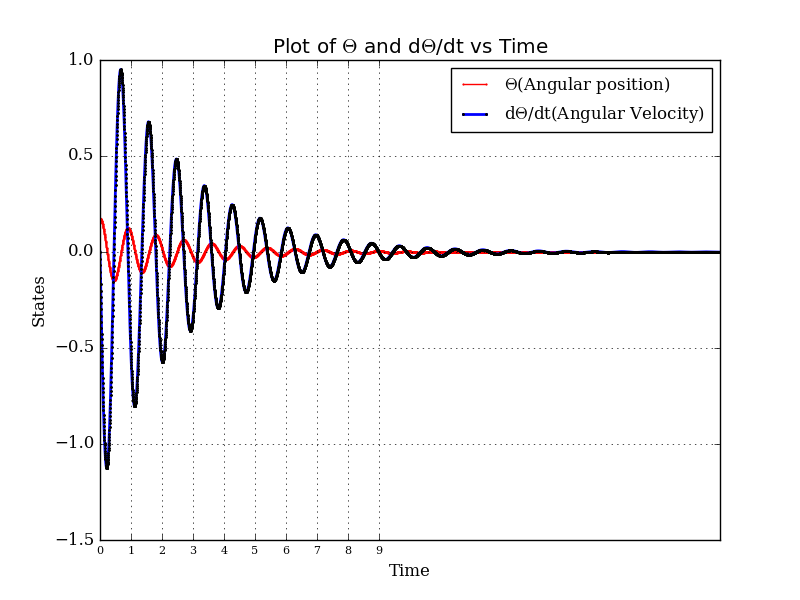
\includegraphics[scale=0.5]{fig(1).png}
    \caption{Plot of states versus time by 153070032}
\end{figure}
\begin{figure}[H]
    \centering
    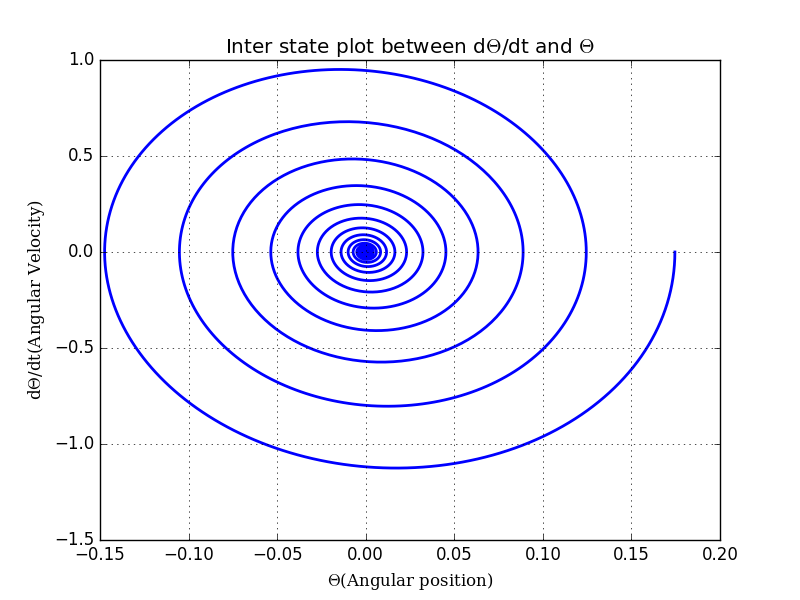
\includegraphics[scale=0.5]{fig(2).png}
    \caption{Omega vs Theta by 153070032}
\end{figure}
\bibliography{153070032}
\addcontentsline{toc}{section}{References}
\bibliographystyle{plain}
\end{document}
\grid
